% !TEX root = main.tex
\section{Theory and Related Work}
\label{sec:theory}

The PDIA posterior distribution takes the form of an infinite mixture of PDFAs.  In practice, we run a sampler for some number of iterations and approximate the posterior with a finite mixture of PDFAs.  For this reason, we now consider the expressive power of finite mixtures of PDFAs.  We show that they are strictly more expressive than PDFAs, but strictly less expressive than hidden Markov models.

%The natural generalization of PDFAs is to probabilistic {\em non}-deterministic finite automata (PNFA), which are like PDFAs except the transition function $\delta$ is stochastic.  That is, given a state and a symbol emitted from that state, the next state is chosen from distribution over successor states.  \comment{If all successor state distributions assign mass to only one state, the PNFA is a PDFA.}  PNFAs have the same expressive power as hidden Markov models: for any HMM there is a PNFA that defines the same distribution over strings, and vice versa \cite{Dupont2005}.

\begin{figure}[htbp]
\begin{center}
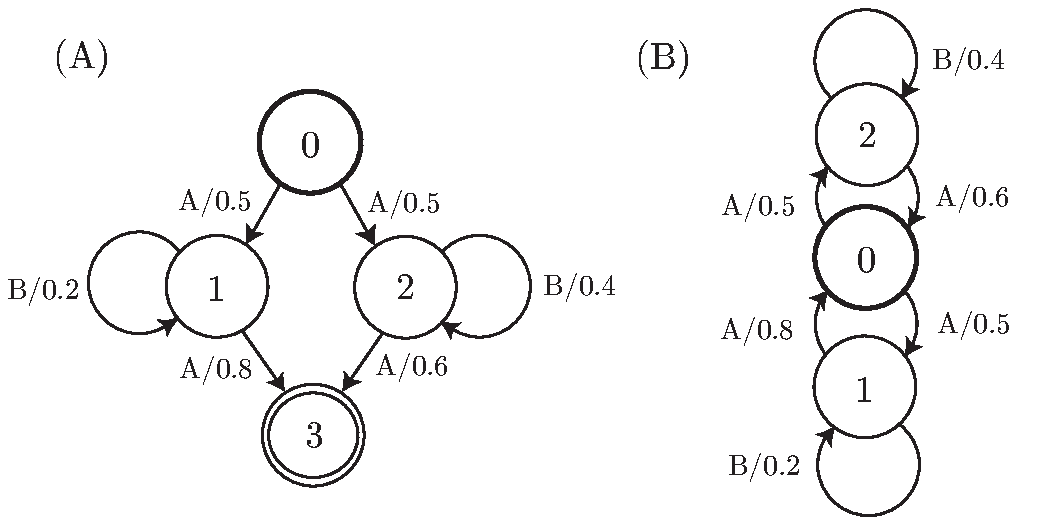
\includegraphics[scale=0.4]{pnfa.pdf}
\caption{Two PNFAs outside the class of PDFAs.  (a) can be represented by a mixture of two PDFAs, one following the right branch from state 0, the other following the left branch.  (b), in contrast, cannot be represented by any finite mixture of PDFAs.}
\label{pnfa}
\end{center}
\end{figure}

Probabilistic {\em non}-deterministic finite automata (PNFA) are a strictly larger model class than PDFAs.  For example, the PNFA in \ref{pnfa}(a) cannot be expressed as a PDFA.  However, it can be expressed as a mixture of two PDFAs, one with $Q = \{q_0,q_1,q_3\}$ and the other with $Q = \{q_0,q_2,q_3\}$.  Thus mixtures of PDFAs are a strictly larger model class than PDFAs.  In general, any PNFA where the nondeterministic transitions can only be visited once can be expressed as a mixture of PDFAs.  However, if we replace transitions to $q_3$ with transitions to $q_0$, as in \ref{pnfa}(b), there is no longer any equivalent finite mixture of PDFAs, since the nondeterministic branch from $q_0$ can be visited an arbitrary number of times.    \comment{This can be done by splitting a PNFA with $n$ possible values for $\delta(q_i,s_j)$ into $n$ PNFAs with deterministic $\delta(q_i,s_j)$, and repeating until all transitions are deterministic.  This includes the class of acyclic PNFAs as a trivial subset.  If there are any cycles that return to a state with nondeterministic transition, there is no equivalent finite mixture of PDFAs.}

\comment{It is important to note that the algorithm presented here will not always discover the appropriate mixture of PDFAs if the data-generating mechanism is like that in \ref{pnfa}(a).  Our intent is to clarify where the class of models that includes our posterior estimate falls in the Chomsky hierarchy, rather than to make any claim as to what class of models can be efficiently learned.}

Previous work on PDFA induction has focused on accurately discovering model structure when the true generative mechanism is a PDFA.  State merging algorithms do this by starting with the trivial PDFA that only accepts the training data and merging states that pass a similarity test \cite{Carrasco1994,Thollard2000}, and have been proven to identify the correct model in the limit of infinite data.  State splitting algorithms start at the opposite extreme, with the trivial single-state PDFA, and split states that pass a difference test \cite{Ron1996,Shalizi2004}.  These algorithms return only a deterministic estimate, while ours naturally expresses uncertainty about the learned model.

To test if we can learn the generative mechanism given our inductive bias, we trained the PDIA on data from three synthetic grammars: the even process \cite{Shalizi2004}, the Reber grammar \cite{Reber1967} and the Feldman grammar \cite{Feldman1966}, which have up to 7 states and 7 symbols in the alphabet.  Performance was good, even on small data.  Details are given in the appendix.



\begin{figure}[htbp]
<<<<<<< HEAD
\begin{center}
\subfigure[Even Process]{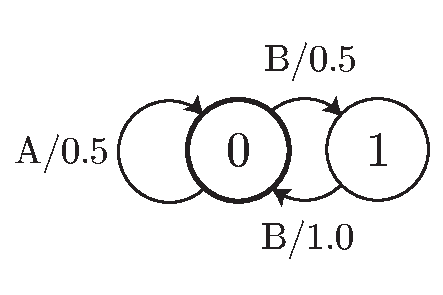
\includegraphics[scale=0.8]{even.pdf}} \\
\subfigure[Reber Grammar]{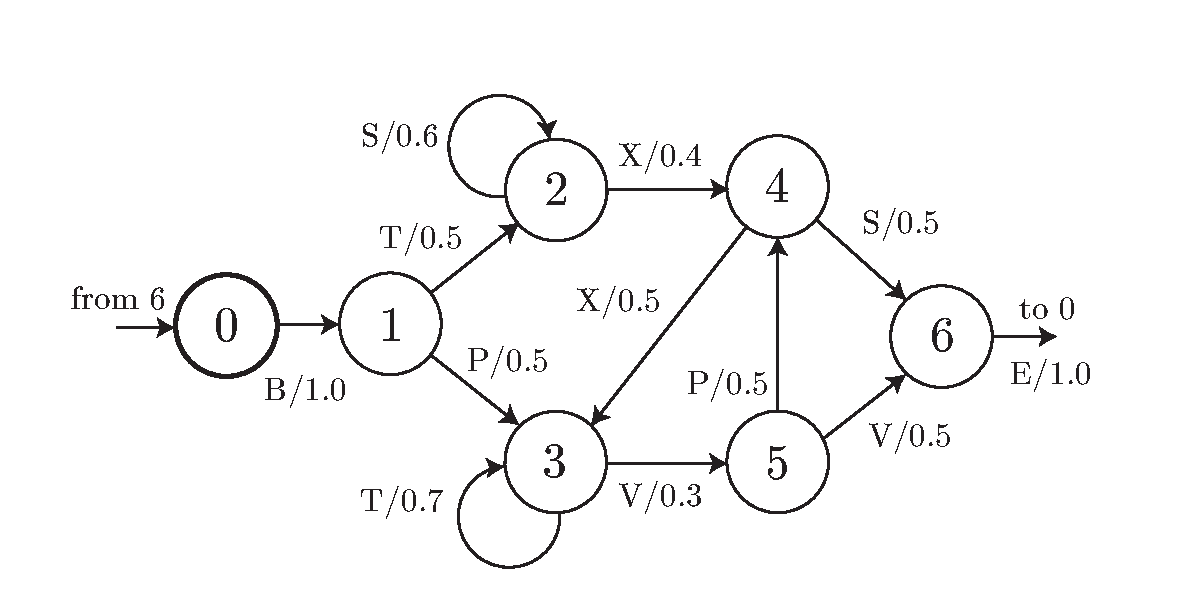
\includegraphics[scale=0.6]{reber.pdf}} \\
\subfigure[Feldman Grammar]{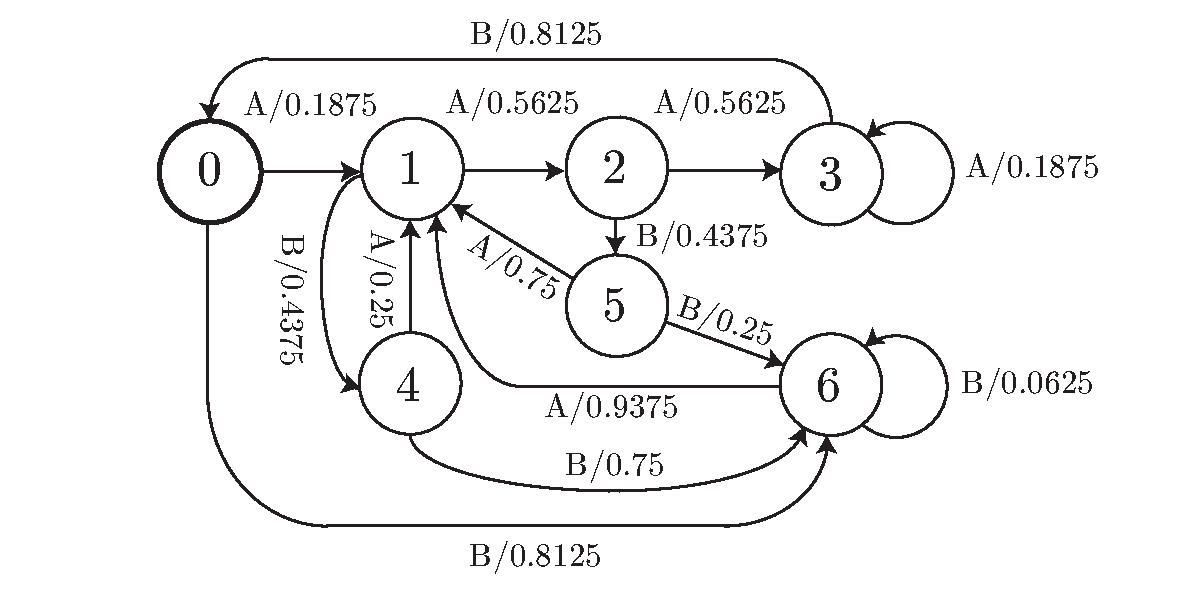
\includegraphics[scale=0.6]{feldman.pdf}}
\label{fig:synthetic_grammar}
\caption{Synthetic grammars used in Figure \ref{fig:synth_results}}
\end{center}
=======
\centering
\subfigure[Even]{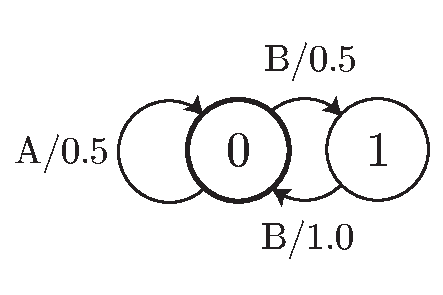
\includegraphics[scale=0.32]{even.pdf}\label{subfig:even}} \hspace{-.55cm} 
\subfigure[Reber]{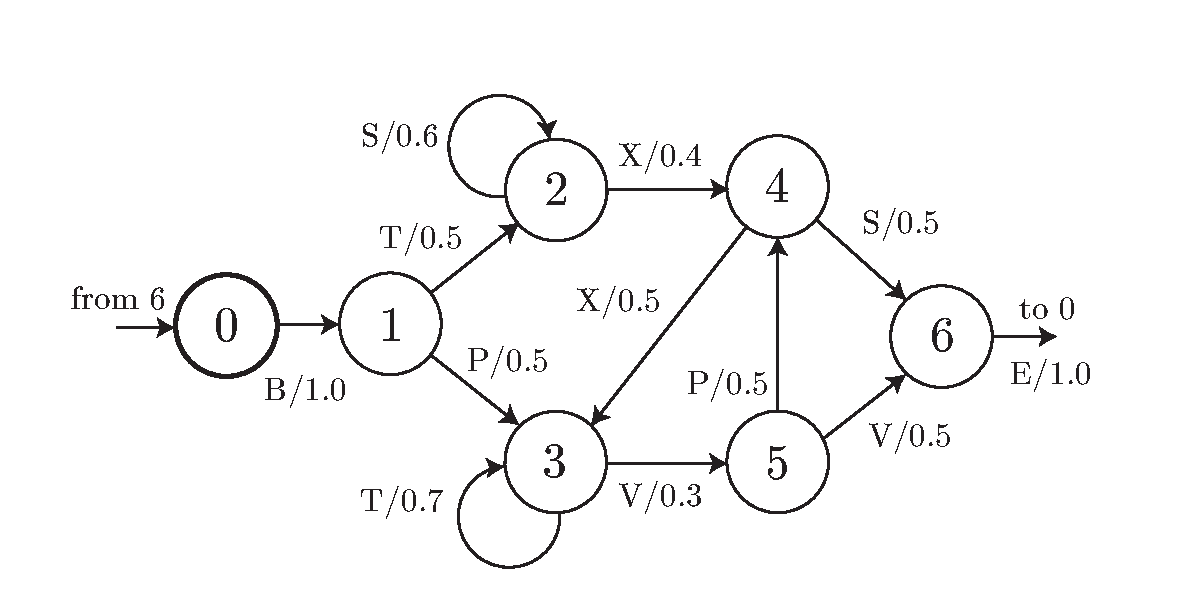
\includegraphics[scale=0.32]{reber.pdf}\label{subfig:reber}}  \hspace{-1.25cm} 
\subfigure[Feldman]{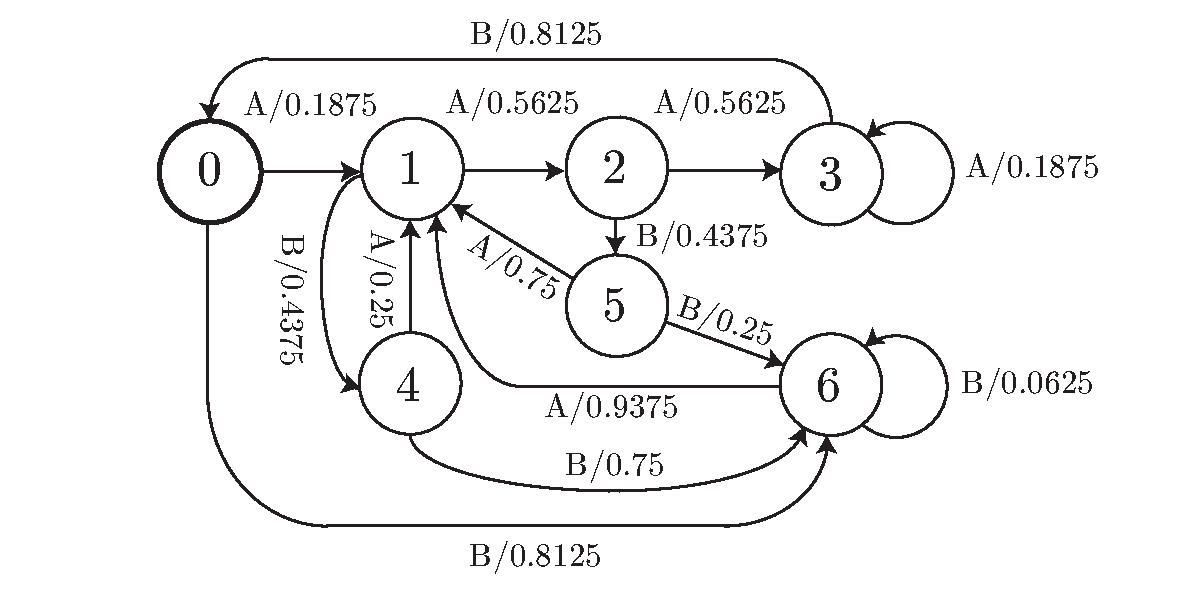
\includegraphics[scale=0.32]{feldman.pdf}\label{subfig:feldman}} \\
\subfigure[Posterior marginal PDIA state cardinality distribution]{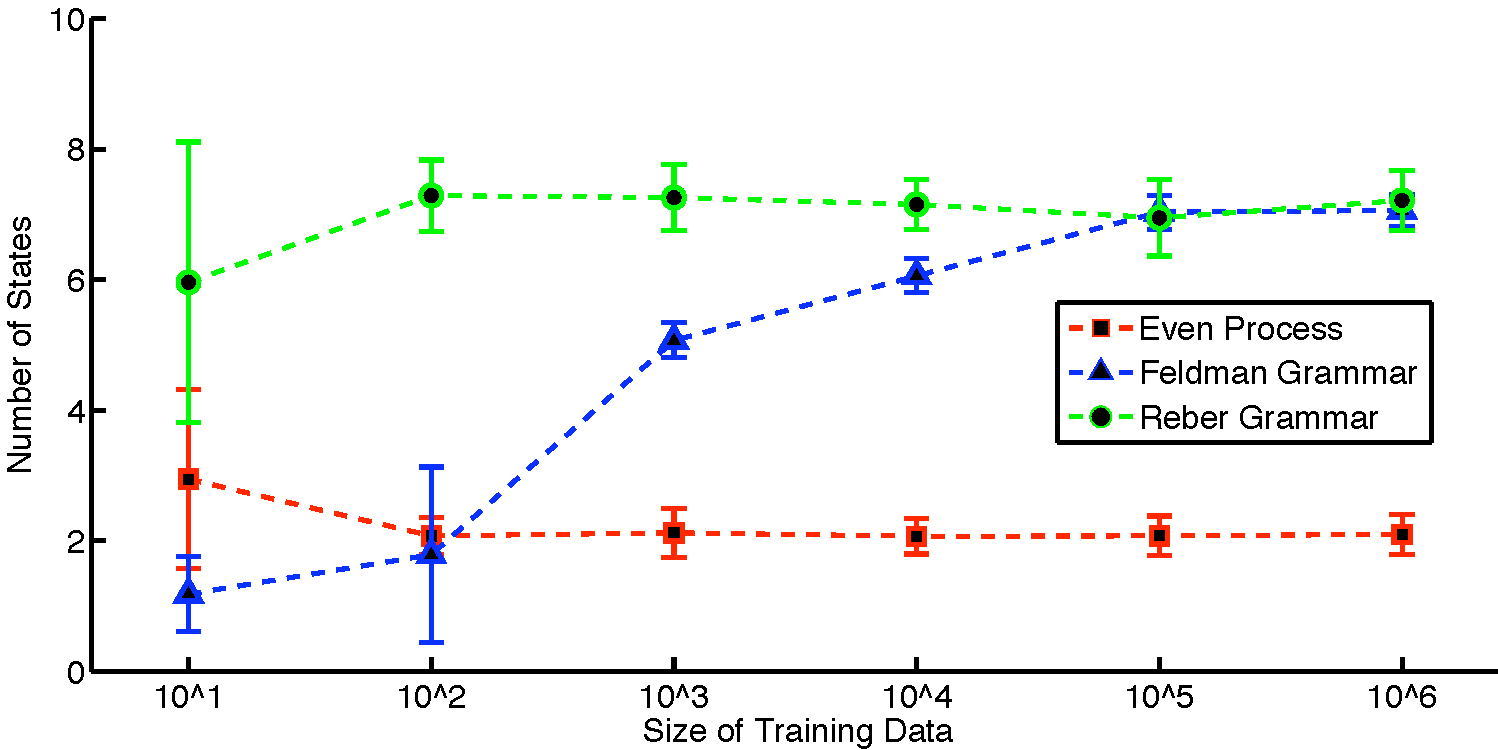
\includegraphics[scale=0.3]{results/syntheticResults.pdf}\label{subfig:posterior}}
\label{fig:synthetic_grammar_and_synth_results}
\caption{Three synthetic PDFAs: \subref{subfig:even} even process, \subref{subfig:reber} Reber grammar, \subref{subfig:feldman} Feldman grammar.  \subref{subfig:posterior} posterior mean and standard deviation of number of states discovered during PDIA inference for varying amounts of data generated by each of the synthetic PDFAs.  PDIA inference discovers PDFAs with the correct number of states}
>>>>>>> 6816a6b84156c68cf30e26d154db4836531ea7c3
\end{figure}